\documentclass[3p,times]{elsarticle}

\usepackage[T1]{fontenc}
\usepackage[utf8]{inputenc}
\usepackage{amsmath,amssymb,amsthm}
\usepackage{graphicx}
\usepackage{booktabs}
\usepackage{multirow}
\usepackage{placeins}
\usepackage{float}
\usepackage{algorithm}
\usepackage{algpseudocode}
\usepackage{hyperref}
\hypersetup{colorlinks=true,linkcolor=blue,citecolor=blue,urlcolor=blue}
\usepackage[capitalise,noabbrev]{cleveref}
\usepackage{xr}
\externaldocument{main}

\newtheorem{proposition}{Proposition}
\newtheorem{lemma}{Lemma}
\newtheorem{definition}{Definition}
\newtheorem{assumption}{Assumption}

\biboptions{numbers,sort&compress}
\setlength{\emergencystretch}{2em}
\journal{Engineering Applications of Artificial Intelligence}

\floatplacement{table}{H}
\floatplacement{figure}{H}

\begin{document}

\begin{frontmatter}
\title{Supplementary Material: Alert-Budgeted Clinical Early Warning}
\author{Anonymous Author(s)}
\begin{abstract}
This supplement reports secondary analyses referenced from the main manuscript: target label cost, seed-level utility-ranked selection, proofs, backbone and bootstrap comparisons, partial clinical-instrument baselines, target adaptation, ablations, and expected calibration error. It is intended to be read alongside the main text.
\end{abstract}
\end{frontmatter}

\section{Cohort Audit}
\label{sec:supp-cohort}

\begin{table}[H]
\centering
\caption{Public 2019 cohort audit after downloading and checksum verification. Percentages for observed variables are the fraction of records with at least one non-missing value. The two sites are separate hospital systems.}
\label{tab:cohort}
\begin{tabular}{lrr}
\toprule
Quantity & Site A & Site B \\
\midrule
Records & 20{,}336 & 20{,}000 \\
Positive records & 1{,}790 & 1{,}142 \\
Left-censored records & 203 & 223 \\
Identifiable pre-onset events & 1{,}587 & 919 \\
Median observed stay (h) & 39 & 38 \\
EtCO$_2$ observed (\%) & 0.0 & 7.6 \\
Temperature observed (\%) & 33.8 & 33.9 \\
Lactate observed (\%) & 3.4 & 1.9 \\
\bottomrule
\end{tabular}
\end{table}


\section{Target-Site Recalibration}
\label{sec:supp-target}

The no-recalibration audit establishes that the source threshold does not travel, but it does not quantify how much of the loss is recoverable by adaptation. We split target B into subject-disjoint calibration and test halves (7,412 patients each; on average 354 calibration events and 337 test events over three seeds), recalibrated the same policy family on B calibration labels, and evaluated it on the B test half. This is an oracle diagnostic: target labels are used for threshold selection, so it is not a deployable label-free procedure and must not be compared with the primary external audit as if it were one. Table~\ref{tab:target} reports the result for the logistic scorer. At 1 alarm per patient-day, target calibration raises mean B sensitivity from $0.294\pm0.082$ to $0.497\pm0.022$ and the realised rate from $0.270\pm0.065$ to $0.616\pm0.058$; at 0.25 per day it raises sensitivity from $0.073\pm0.026$ to $0.218\pm0.036$ at a realised rate of $0.159\pm0.009$. The recovery is real but partial, and it is purchased with a higher alarm load and a higher patient-violation fraction because the target-calibrated threshold is lower. The single-seed GRU diagnostic shows the same direction ($0.314$ to $0.493$ at 1 per day). At 2 per day the target-recalibrated selector hits the threshold-grid floor: sensitivity saturates at $0.724\pm0.056$ while the realised rate rises to $1.466\pm0.260$, so the diagnostic identifies a range where adaptation matters rather than a universal gain.

\begin{table}[H]
\centering
\caption{Target-site recalibration diagnostic for the prefix logistic scorer, mean $\pm$ sample standard deviation over three source seeds. The target hospital is split 50/50 into subject-disjoint calibration and test halves; the calibration half uses target labels to select the threshold. Sensitivity and realised alarm rate are evaluated on the target test half (7,412 patients, about 337 events). This is an oracle-style target-calibrated reference estimate, not a deployable label-free procedure.}
\label{tab:target}
\small
\begin{tabular}{lcccc}
\toprule
 & \multicolumn{2}{c}{No recalibration} & \multicolumn{2}{c}{Target recalibrated} \\
\cmidrule(lr){2-3}\cmidrule(lr){4-5}
Budget & Sens. & Rate & Sens. & Rate \\
\midrule
0.25 & $0.073\pm0.026$ & $0.039\pm0.014$ & $0.218\pm0.036$ & $0.159\pm0.009$ \\
0.50 & $0.173\pm0.074$ & $0.118\pm0.043$ & $0.358\pm0.031$ & $0.360\pm0.019$ \\
1.00 & $0.294\pm0.082$ & $0.270\pm0.065$ & $0.497\pm0.022$ & $0.616\pm0.058$ \\
2.00 & $0.544\pm0.072$ & $0.744\pm0.165$ & $0.724\pm0.056$ & $1.466\pm0.260$ \\
\bottomrule
\end{tabular}
\end{table}


\section{Utility-Ranked Selection: Seed-Level Results}
\label{sec:supp-ucrc}

Table~\ref{tab:ucrc-seeds} reports the utility-ranked CRC (U-CRC) selector for every source seed rather than only the primary seed. The validation rate is computed on the disjoint validation partition used to rank calibration-feasible thresholds; the internal and external rates and utilities are evaluated on the held-out A test and transported B sets. At 2 per patient-day U-CRC selects the same threshold as at 1 per day for all three seeds, which is the intended refusal to spend a loose budget rather than a grid artefact. Internal utility varies from 0.613 to 0.932 at the loose budget, so the seed-0 value in the main table should not be read as a mean. U-CRC remains a deployment heuristic: the validation lower bound reduces variance-driven selection but provides no finite-sample utility guarantee.

\begin{table}[H]
\centering
\caption{Seed-level U-CRC results. ``Val.'' is the mean alarm rate on the validation partition; ``Int.'' and ``Ext.'' are the held-out A test and transported B evaluation. Utility is the official 2019 challenge score (inactive $=0$, oracle $=1$).}
\label{tab:ucrc-seeds}
\small
\resizebox{\columnwidth}{!}{%
\begin{tabular}{cccccccc}
\toprule
 & & \multicolumn{3}{c}{Internal A} & \multicolumn{3}{c}{External B} \\
\cmidrule(lr){3-5}\cmidrule(lr){6-8}
Budget & Seed & Val. rate & Rate & Utility & Rate & Utility \\
\midrule
0.25 & 0 & 0.273 & 0.239 & 0.691 & 0.115 & 0.244 \\
0.25 & 1 & 0.207 & 0.208 & 0.493 & 0.055 & 0.138 \\
0.25 & 2 & 0.252 & 0.256 & 0.499 & 0.095 & 0.148 \\
0.50 & 0 & 0.479 & 0.450 & 0.910 & 0.231 & 0.270 \\
0.50 & 1 & 0.375 & 0.360 & 0.597 & 0.104 & 0.195 \\
0.50 & 2 & 0.444 & 0.465 & 0.799 & 0.177 & 0.255 \\
1.00 & 0 & 0.668 & 0.631 & 0.932 & 0.348 & 0.278 \\
1.00 & 1 & 0.515 & 0.479 & 0.613 & 0.151 & 0.246 \\
1.00 & 2 & 0.896 & 0.925 & 0.875 & 0.393 & 0.233 \\
2.00 & 0 & 0.668 & 0.631 & 0.932 & 0.348 & 0.278 \\
2.00 & 1 & 0.515 & 0.479 & 0.613 & 0.151 & 0.246 \\
2.00 & 2 & 0.896 & 0.925 & 0.875 & 0.393 & 0.233 \\
\bottomrule
\end{tabular}}
\end{table}


\section{Detailed Proofs}
\label{sec:supp-proofs}

\begin{proof}
For each fixed $\lambda$, the relevant one-sided Hoeffding inequality is
\begin{equation*}
\Pr\{R(\lambda)-\widehat R_n(\lambda)>\epsilon\}
 \le\exp(-2n\epsilon^2/L_{\max}^2).
\end{equation*}
Setting $\epsilon=L_{\max}\sqrt{\log(|\Lambda|/\alpha)/(2n)}$ and applying a union bound gives simultaneous upper bounds $R(\lambda)\le\widehat R_n(\lambda)+\epsilon$ for all grid policies with probability at least $1-\alpha$. On that event, any policy selected from the feasible set satisfies $R(\widehat\lambda)\le B$. If the feasible set is empty, the fallback has identically zero loss and hence satisfies the budget without a concentration argument. Thus a budget violation can occur only on the failure event of the simultaneous upper bounds, which has probability at most $\alpha$.
\end{proof}

\begin{proof}
For a fixed $\lambda$, the random variables $L_i(\lambda)$ lie in $[0,L_{\max}]$ and are independent across subjects. The empirical-Bernstein inequality of Maurer and Pontil \citep{maurer2009empirical} with failure probability $\delta=\alpha/|\Lambda|$ gives, with probability at least $1-\delta$,
\begin{equation*}
R(\lambda)\le\widehat R_n(\lambda)
+\widehat\sigma_n(\lambda)\sqrt{\frac{2\log(2/\delta)}{n}}
+\frac{7L_{\max}\log(2/\delta)}{3(n-1)}.
\end{equation*}
Substituting $\delta=\alpha/|\Lambda|$ yields the radius in \eqref{eq:bernstein}. A union bound over the $|\Lambda|$ fixed grid points makes these inequalities simultaneous with probability at least $1-\alpha$. On that event, every policy in the feasible set of \eqref{eq:lambda-eb} satisfies $R(\lambda)\le B$; the no-alarm fallback has zero loss. Thus a budget violation can occur only on the union-bound failure event, whose probability is at most $\alpha$.
\end{proof}

\begin{proof}
For a fixed $\lambda$, exchangeability of the $n+1$ calibration and deployment losses gives $\mathbb{E}[\widehat R_{n+1}(\lambda)]=R(\lambda)$. The CRC correction is the finite-sample version of the same identity applied to the order statistic that includes the deployment point; the selected threshold is the smallest one whose corrected empirical loss is below $B$. The standard conformal risk control argument then yields $\mathbb{E}[R(\widehat\lambda_{\mathrm{CRC}})]\le B$ for any bounded monotone loss, including the patient-blocked alarm rate. The finite grid is handled by the same selection rule; no union bound is required because the guarantee is in expectation rather than simultaneously over the grid.
\end{proof}

\begin{proof}
Conditional on the randomisation draw, the loss is the corresponding deterministic loss; taking expectation over the draw gives the convex combination. The augmented-family statement follows by applying Proposition~\ref{prop:validity} or~\ref{prop:eb} to the enlarged fixed grid.
\end{proof}


\section{Target Label Cost}
\subsection{How Many Target Labels Are Needed?}
\label{sec:label-budget}

The single 50/50 target diagnostic answers whether adaptation can recover sensitivity, but not how much target annotation that recovery requires. We therefore fix the target test half and draw nested calibration subsets from the remaining target pool at 5\%, 10\%, 25\% and 50\% of all eligible target subjects. Each subset is drawn without replacement from the same shuffled pool, so the curve isolates calibration-set size rather than a change of test patients. The source threshold is evaluated on the same test half as the no-recalibration reference, and every recalibrated threshold is selected by the same patient-blocked procedure used elsewhere.


\begin{figure}[H]
\centering
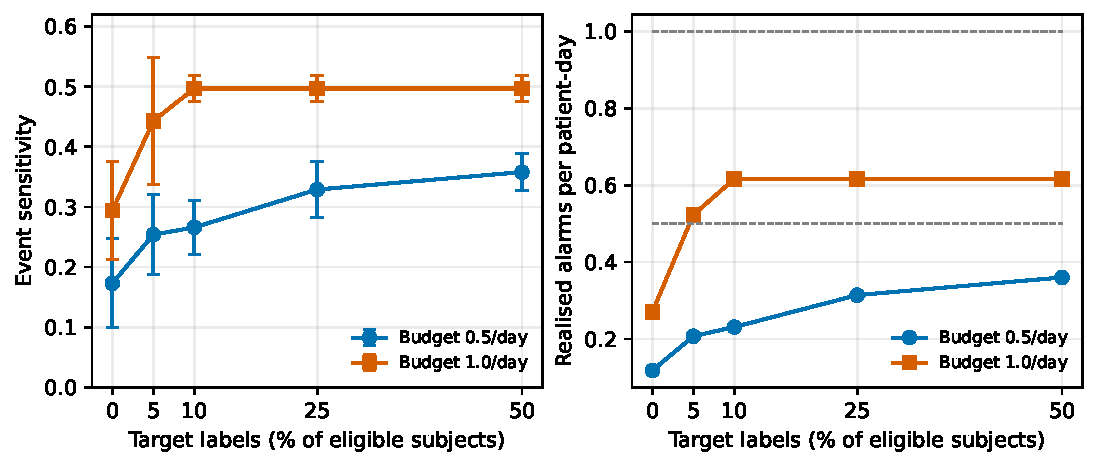
\includegraphics[width=\linewidth]{figures/label_budget.pdf}
\caption{Target label-budget curve for the logistic scorer, averaged over three source seeds. Left: event sensitivity versus the percentage of eligible target subjects used for threshold calibration; error bars are sample standard deviations over seeds. Right: realised alarms per patient-day against the requested budget (dashed lines), showing that label cost and operating point interact. The zero-label point applies the source threshold without target calibration.}
\label{fig:label-budget}
\end{figure}

Table~\ref{tab:label-budget} reports the resulting label-budget curve for the logistic scorer, averaged over the three source seeds. At the 1-per-day budget, 741 target patients (5\% of the eligible cohort, about 34 calibration events) raise mean test sensitivity from $0.294\pm0.082$ to $0.443\pm0.106$, which is most of the $0.497\pm0.022$ obtained with the full calibration pool. At 10\% (1,482 patients, about 72 events), the curve reaches the full-pool value, and additional labels do not change the selected threshold on these seeds. The lower budget behaves differently: at 0.5 per day, 5\% reaches $0.254\pm0.066$ against a full-pool value of $0.358\pm0.031$, 25\% reaches $0.329\pm0.046$, and only the largest subset closes the gap. A hospital that needs a low alarm load therefore needs more target labels than one operating at 1 per patient-day, because the threshold sits in a denser part of the score distribution where small calibration errors move more patients across the boundary.

\begin{table}[H]
\centering
\caption{Target label-budget curve for the prefix logistic scorer, mean $\pm$ sample standard deviation over three source seeds. The target test half contains 7,412 patients and about 337 events. ``None'' applies the source threshold without target labels. The remaining rows recalibrate on a nested subset of the target calibration pool; labels and rates are evaluated on the same test half. This is an oracle-style label-budget diagnostic, not a deployable label-free procedure.}
\label{tab:label-budget}
\small
\begin{tabular}{lcccccc}
\toprule
 & & & \multicolumn{2}{c}{Budget 0.5} & \multicolumn{2}{c}{Budget 1.0} \\
\cmidrule(lr){4-5}\cmidrule(lr){6-7}
Labels & Patients & Events & Sens. & Rate & Sens. & Rate \\
\midrule
None & 0 & 0 & $0.173\pm0.074$ & $0.118$ & $0.294\pm0.082$ & $0.270$ \\
5\% & 741 & 34 & $0.254\pm0.066$ & $0.207$ & $0.443\pm0.106$ & $0.523$ \\
10\% & 1,482 & 72 & $0.266\pm0.045$ & $0.231$ & $0.497\pm0.022$ & $0.616$ \\
25\% & 3,706 & 176 & $0.329\pm0.046$ & $0.314$ & $0.497\pm0.022$ & $0.616$ \\
50\% & 7,412 & 354 & $0.358\pm0.031$ & $0.360$ & $0.497\pm0.022$ & $0.616$ \\
\bottomrule
\end{tabular}
\end{table}

Two cautions follow from the table. First, the 5\% point has the widest seed-to-seed spread at 1 per day ($\pm0.106$ versus $\pm0.022$ for the full pool), so a small target set can recover the mean operating point while remaining unstable across source models. Second, the curve is conditional on the target split and on the policy family; it measures threshold-selection label cost, not the cost of retraining the scorer. The result is an engineering signal about the label cost of a \emph{certified} target threshold; the label-free rate-matching rule in \cref{sec:adaptation} can recover the operating point on this cohort without target labels, but it controls the alarm rate rather than the risk and therefore does not replace this curve when a finite-sample guarantee is required.


\section{Backbone and Bootstrap Comparisons}
\subsection{Backbone Comparison at a Fixed Alarm Budget}
\label{sec:models}

A budget curve is only as useful as the scores it ranks. Table~\ref{tab:model-comparison} therefore compares the three backbones at the 1-per-patient-day operating point, holding the policy family, support bound and threshold grid fixed. At site A the GRU has the highest mean sensitivity ($0.684\pm0.006$), followed by LightGBM ($0.661\pm0.042$) and the prefix logistic model ($0.585\pm0.020$). At site B the ordering changes: LightGBM reaches $0.540\pm0.071$, the GRU $0.375\pm0.078$, and the logistic model $0.315\pm0.062$. The LightGBM advantage is not a free lunch, because its B alarm rate is also higher ($0.410\pm0.156$ versus $0.276\pm0.063$ for logistic and $0.328\pm0.164$ for the GRU), but all three policies remain below the requested B budget of 1 per day. A stronger tabular scorer therefore narrows the transport gap without eliminating it.

\begin{table}[H]
\centering
\caption{Backbone comparison at the 1-per-patient-day operating point, mean $\pm$ sample standard deviation over three seeds. The threshold is calibrated on site A and applied unchanged to site B. Rates are realised alarms per patient-day; the requested budget is 1.0. LightGBM is a stronger tabular baseline, not a tuned state-of-the-art model.}
\label{tab:model-comparison}
\small
\begin{tabular}{lcccc}
\toprule
 & \multicolumn{2}{c}{Site A} & \multicolumn{2}{c}{Site B} \\
\cmidrule(lr){2-3}\cmidrule(lr){4-5}
Model & Sens. & Rate & Sens. & Rate \\
\midrule
Prefix logistic & $0.585\pm0.020$ & $0.651\pm0.022$ & $0.315\pm0.062$ & $0.276\pm0.063$ \\
Masked GRU & $0.684\pm0.006$ & $0.635\pm0.121$ & $0.375\pm0.078$ & $0.328\pm0.164$ \\
LightGBM & $0.661\pm0.042$ & $0.655\pm0.147$ & $0.540\pm0.071$ & $0.410\pm0.156$ \\
\bottomrule
\end{tabular}
\end{table}

The seed-0 patient-block bootstrap makes the LightGBM--logistic contrast concrete without turning it into a universal ranking. At site B and 1 per day, the paired LightGBM-minus-logistic sensitivity difference is $0.081$ with 95\% interval $[0.027,0.133]$ and Holm-adjusted $p=0.066$; the alarm-rate difference is $-0.087$ with interval $[-0.105,-0.069]$ and adjusted $p=0.036$, because LightGBM selects a lower threshold and alarms less often on the shifted distribution. On site A the same contrast is not significant after correction, so the external comparison is the relevant one. The sensitivity advantage is consistent but not decisive after correction, while the lower alarm rate is clearer. The result supports a modest claim: backbone quality matters for transport, but it changes the level of the frontier rather than removing the need for target calibration. A hospital still cannot infer its realised alarm load from an A-calibrated threshold alone.

\subsection{Patient-Block Uncertainty}
\label{sec:uncertainty}

Seed-to-seed standard deviations describe calibration variability, not sampling uncertainty on the target population. We therefore resample whole B subjects with replacement 2{,}000 times at the 1-per-day operating point and recompute sensitivity, realised rate and patient-violation fraction on each replicate. Resampling subjects rather than hours preserves the within-patient dependence that the calibration argument is built on. Table~\ref{tab:bootstrap} reports the seed-0 intervals and paired differences against the blocked prefix-logistic policy; Holm adjustment covers the six model--procedure rows and three metrics.

\begin{table}[H]
\centering
\caption{Patient-block bootstrap at the 1-per-patient-day operating point on site B, seed 0, 2{,}000 resamples. Intervals are 95\% percentile intervals. $\Delta$Sens is the paired difference against the blocked prefix-logistic policy; $p_{\mathrm{Holm}}$ is adjusted across the reported rows and metrics. The global rows use a point-estimate threshold and are workload comparators, not certified policies.}
\label{tab:bootstrap}
\scriptsize
\setlength{\tabcolsep}{3pt}
\begin{tabular}{lcccc}
\toprule
Policy & Sens. [95\% CI] & Rate [95\% CI] & $\Delta$Sens [95\% CI] & $p_{\mathrm{Holm}}$ \\
\midrule
Prefix logistic, blocked & $0.382$ [0.348, 0.417] & $0.348$ [0.333, 0.362] & -- & -- \\
Prefix logistic, global & $0.482$ [0.443, 0.519] & $0.549$ [0.531, 0.568] & $+0.100$ [0.049, 0.152] & 0.040 \\
Masked GRU, blocked & $0.326$ [0.291, 0.359] & $0.209$ [0.198, 0.219] & $-0.056$ [-0.106, -0.009] & 0.288 \\
Masked GRU, global & $0.408$ [0.370, 0.445] & $0.343$ [0.329, 0.357] & $+0.026$ [-0.029, 0.076] & 1.000 \\
LightGBM, blocked & $0.463$ [0.427, 0.499] & $0.260$ [0.250, 0.272] & $+0.081$ [0.027, 0.133] & 0.066 \\
LightGBM, global & $0.537$ [0.501, 0.574] & $0.400$ [0.387, 0.413] & $+0.155$ [0.103, 0.208] & 0.033 \\
\bottomrule
\end{tabular}
\end{table}

Three patterns survive the intervals. First, the blocked prefix policy is conservative on this target: its mean rate is $0.348$ with interval $[0.333,0.361]$, well below the requested 1 per day, and its sensitivity interval is $[0.348,0.417]$. Second, the global point-estimate threshold raises sensitivity by $0.100$ but also raises the realised rate by $0.201$ alarms per patient-day and the patient-violation fraction from $0.122$ to $0.190$; the gain is a change of operating point, not a free improvement in ranking. Third, LightGBM's blocked policy reaches $0.463$ sensitivity at $0.260$ alarms per day, a paired gain of $0.081$ over the blocked logistic policy with interval $[0.027,0.133]$; the Holm-adjusted $p=0.066$ is not significant at the 0.05 level, so this is a consistent but not decisive advantage. The GRU difference is negative at this operating point and is also not significant after Holm adjustment, which is why the GRU is presented as a secondary check rather than a demonstrated improvement.

These intervals are conditional on one target split and one seed; they quantify target sampling noise, not source-seed or hospital-level variability. They also do not cover the oracle target-calibration analysis, which uses target labels and is reported separately. The practical reading is therefore limited but useful: at a fixed 1-per-day request, the choice of backbone and threshold procedure can move B sensitivity by roughly ten percentage points, while the realised rate remains below the request for every certified row in the table.


\section{Clinical-Instrument Baselines}
\subsection{Partial Clinical-Instrument Baselines}
\label{sec:clinical}

A learned score is not the only way to operate an alarm policy, so we calibrated partial NEWS, SIRS and qSOFA on the same A calibration subjects and evaluated them at the same requested budgets. Table~\ref{tab:clinical} reports the 1-per-day operating point. The instruments are coarse integer scores, and the calibration grid is limited to their attainable values; qSOFA, for example, has only three levels, so the selector can miss a requested budget by a wide margin or return the no-alarm fallback. On site A, NEWS reaches $0.399$ sensitivity at $0.730$ alarms per day, SIRS reaches $0.470$ at $0.796$, and qSOFA reaches only $0.220$ at $0.492$. The learned logistic policy is more sensitive at a lower rate ($0.585$ at $0.651$), and LightGBM is higher still ($0.661$ at $0.655$).

\begin{table}[H]
\centering
\caption{Partial clinical-instrument baselines at the 1-per-patient-day operating point. Thresholds are calibrated on site A and applied unchanged to site B. NEWS, SIRS and qSOFA omit components unavailable in the 2019 release and are research-only partial instruments. qSOFA has a three-level grid, so its realised rate is far from the request.}
\label{tab:clinical}
\small
\begin{tabular}{lcccc}
\toprule
 & \multicolumn{2}{c}{Site A} & \multicolumn{2}{c}{Site B} \\
\cmidrule(lr){2-3}\cmidrule(lr){4-5}
Policy & Sens. & Rate & Sens. & Rate \\
\midrule
Prefix logistic & $0.585$ & $0.651$ & $0.315$ & $0.276$ \\
LightGBM & $0.661$ & $0.655$ & $0.540$ & $0.410$ \\
Partial NEWS & $0.399$ & $0.730$ & $0.449$ & $0.586$ \\
Partial SIRS & $0.470$ & $0.796$ & $0.424$ & $0.493$ \\
Partial qSOFA & $0.220$ & $0.492$ & $0.240$ & $0.327$ \\
\bottomrule
\end{tabular}
\end{table}

The external ordering is not the same as the internal one. NEWS and SIRS beat the source-threshold logistic policy on site B ($0.449$ [0.412, 0.484] and $0.424$ [0.389, 0.461] versus $0.315$), but they do so at higher realised rates ($0.586$ [0.570, 0.602] and $0.493$ [0.478, 0.508] versus $0.276$), and neither reaches the LightGBM sensitivity of $0.540$ at $0.410$. The paired sensitivity differences against the blocked logistic policy are $+0.067$ [0.016, 0.118] for NEWS, $+0.042$ [-0.008, 0.093] for SIRS and $-0.142$ [-0.190, -0.095] for qSOFA; only the qSOFA loss survives Holm correction, and all three clinical instruments increase the realised rate. This is a workload comparison, not evidence that the instruments are clinically equivalent: their missing components are systematic, their scores are not probabilities, and their thresholds were selected on A. The result does show that a simple, auditable instrument can be a competitive external baseline once the comparison is made at a declared patient-level alarm budget instead of at an arbitrary threshold.

The coarse grids also expose a practical failure mode that probability-valued scorers hide. At 0.25 per day, qSOFA has no admissible threshold and returns the no-alarm fallback on both sites; at 0.5 per day its only feasible threshold alarms on $0.492$ of A patient-days and $0.327$ of B patient-days. NEWS and SIRS similarly jump between adjacent integer levels, which makes the realised rate a step function of the request. A hospital that needs fine workload control should therefore not rely on an integer instrument alone, even when its discrimination is adequate; the policy layer needs either a richer score or an explicit randomization/utility rule over neighbouring thresholds. These baselines are reported to bound what a simple instrument can do under the same budget protocol, not to propose one for deployment.


\section{Target Adaptation and Ablations}
\label{sec:supp-adaptation}

\subsection{Label-Free Target Adaptation}
\label{sec:adaptation}

The source-threshold audit shows that a threshold trained on A is too quiet on B. A target site that can observe unlabelled traces can still match its requested rate without waiting for outcome labels: it chooses the most aggressive threshold whose empirical alarm rate on a warm-up half of the target subjects is at most the budget, then deploys that threshold on the held-out half. Table~\ref{tab:adaptation} compares this rate-matched rule with source transfer and with an oracle that uses target labels.

\begin{table}[H]
\centering
\caption{Target adaptation on site B, seed 0. The target cohort is split into disjoint warm-up and test halves. ``Source'' applies the A-calibrated threshold; ``rate-matched'' uses no target labels and matches the requested rate on the warm-up half; ``oracle'' recalibrates on target labels. Sensitivity and rate are evaluated on the target test half.}
\label{tab:adaptation}
\small
\begin{tabular}{lcccccc}
\toprule
 & \multicolumn{2}{c}{Source} & \multicolumn{2}{c}{Rate-matched} & \multicolumn{2}{c}{Oracle} \\
\cmidrule(lr){2-3}\cmidrule(lr){4-5}\cmidrule(lr){6-7}
Budget & Sens. & Rate & Sens. & Rate & Sens. & Rate \\
\midrule
0.25 & $0.194$ & $0.094$ & $0.322$ & $0.237$ & $0.261$ & $0.171$ \\
0.50 & $0.261$ & $0.171$ & $0.414$ & $0.356$ & $0.414$ & $0.356$ \\
1.00 & $0.414$ & $0.356$ & $0.620$ & $0.950$ & $0.620$ & $0.950$ \\
2.00 & $0.620$ & $0.950$ & $0.809$ & $1.792$ & $0.809$ & $1.792$ \\
\bottomrule
\end{tabular}
\end{table}

On the target test half the label-free rule recovers the oracle operating point at 0.5, 1 and 2 per day: its threshold coincides with the target-calibrated threshold on the fixed grid. At 1 per day it raises sensitivity on that half from $0.414$ to $0.620$ and the realised rate from $0.356$ to $0.950$, still below the request. The source threshold is quieter on this half than on the full B test set, where the external audit reports $0.315$ sensitivity and a $0.276$ rate, because the warm-up/test partition changes the eligible-event mix. At 0.25 per day it selects a more aggressive threshold than the certified oracle, raising sensitivity from $0.194$ to $0.322$ at a rate of $0.237$ rather than the oracle's $0.261$ at $0.171$. This is a positive engineering result, but it must be read narrowly. The rule is transductive: it uses a warm-up sample from the deployment site, and it controls the alarm rate rather than the risk. If the target case mix changes the relationship between score and event risk, a rate-matched threshold can meet the budget while detecting fewer events. The oracle agreement here is a property of this cohort and this grid, not a general guarantee. The finite-sample certificate still requires labelled target calibration patients; rate matching is a deployment heuristic that can be audited with the operational metrics above.

\subsection{Ablations}
\label{sec:ablation}

One-at-a-time ablations on the primary A split identify which design choices are first-order. The refractory window is one: moving from $\tau=2$ to $\tau=12$ raises sensitivity from $0.518$ to $0.726$ but also raises the patient-violation fraction from $0.167$ to $0.327$ at the 1-per-day budget. The escalation tier is a strong de-alarming control: $\kappa=1$ lowers the realised rate from $0.631$ to $0.472$ and sensitivity from $0.607$ to $0.286$. The lead window changes sensitivity modestly ($0.560$ at 6 hours, $0.607$ at 12, $0.631$ at 24) without changing the threshold. The risk level is second-order on this split: $\alpha=0.05,0.1,0.2$ selects the same threshold, with certified risk changing from $0.844$ to $0.823$. Grid resolution is first-order at the coarse end: 20 thresholds produce a rate of $0.082$ and sensitivity $0.179$, 50 and 100 thresholds produce about $0.44$ and $0.51$, and 200 thresholds recover $0.631$ and $0.607$. The minimum-stay restriction changes both eligibility and the selected threshold: at 6, 12 and 48 hours the sensitivities are $0.627$, $0.655$ and $0.609$ at rates $0.832$, $0.825$ and $0.747$. These results do not justify a universal tuning rule, but they show that the reported operating point depends on declared structural choices, which is why those choices are fixed before calibration and reported with the certificate.

\subsection{Human-Factors Queueing Sensitivity}
\label{sec:queue}

The hourly capacity model above is a deliberately conservative staffing abstraction: one alarm per hour is equivalent to a 60-minute service time, far longer than a typical bedside response. To ground the translation in human-factors data, we add a continuous-time queue in which alarms wait for one of $c$ nurses and service times are exponential with a declared mean. Bridi et al.\ report a median alarm response of about 5 minutes in an intensive-care unit, with more than 60\% of alarms unanswered after 10 minutes during busy periods \citep{bridi2014reaction}. We therefore evaluate mean service times of 5 and 15 minutes; the latter represents detection, travel and bedside confirmation rather than the alarm acknowledgement alone.

\begin{table}[H]
\centering
\caption{Alarm-handling queue on a simulated 20-bed ward with five admissions per day. Service times are exponential; ``Util.'' is nurse utilisation over the 30-day horizon. The 5-minute mean is the median response reported by Bridi et al.; 15 minutes adds travel and confirmation. At 0.25 per day at most 0.7\% of CRC alarms wait more than 5 minutes.}
\label{tab:queue}
\small
\begin{tabular}{lcccccc}
\toprule
Budget & Policy & Service & Util. & $>5$ min & $>10$ min & p95 wait \\
\midrule
1.00 & Blocked & 5 min & $0.032$ & $0.000$ & $0.000$ & $0.0$ \\
1.00 & Blocked & 15 min & $0.095$ & $0.020$ & $0.015$ & $0.0$ \\
1.00 & CRC & 5 min & $0.050$ & $0.022$ & $0.006$ & $0.0$ \\
1.00 & CRC & 15 min & $0.150$ & $0.089$ & $0.070$ & $18.7$ \\
2.00 & Both & 5 min & $0.057$ & $0.024$ & $0.005$ & $0.2$ \\
2.00 & Both & 15 min & $0.171$ & $0.126$ & $0.094$ & $26.8$ \\
\bottomrule
\end{tabular}
\end{table}

Table~\ref{tab:queue} shows that the queue is not saturated even at the loosest budget, but waiting is not negligible once service includes travel. At 1 alarm per patient-day, the blocked policy keeps the fraction waiting more than 10 minutes below 2\% with a 15-minute service mean, whereas CRC reaches 7.0\% and a 95th-percentile wait of 18.7 minutes. At 2 per day both policies produce the same traces on this split and 9.4\% of alarms wait more than 10 minutes with one nurse; a second nurse removes essentially all waits. These fractions are lower than the 60\% unanswered rate in the observational study because our queue assumes perfect work-conserving service and no competing nursing tasks. The comparison is therefore a lower bound on human delay, not a validation of the ward model. Its engineering value is to show that the difference between a 1-per-day and a 2-per-day budget is visible in response latency even when average nurse utilisation is below 20\%, because alarm bursts matter more than the daily mean.


\section{Operational Figure}
\label{sec:supp-figure}

\begin{figure}[H]
\centering
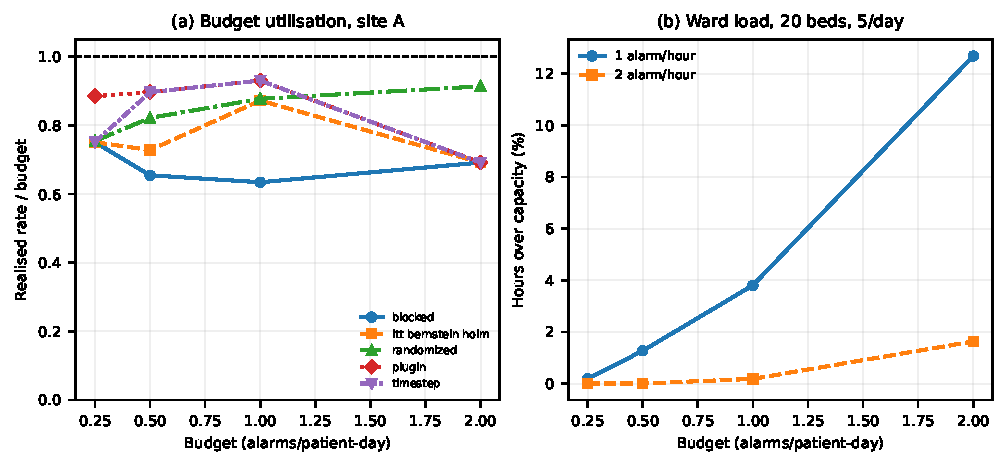
\includegraphics[width=\linewidth]{figures/revision.pdf}
\caption{Operational summary. (a) Realised mean alarm rate divided by the requested budget over ten repeated patient splits on site A; the dashed line is exact utilisation. (b) Percentage of hours in which a simulated 20-bed ward with five admissions per day exceeds its alarm-handling capacity, using the calibrated traces from site A.}
\label{fig:revision}
\end{figure}


\bibliographystyle{elsarticle-num}
\bibliography{refs}

\end{document}
